\subsection{Utilizadores}

% Roles no negócio (administradores e utilizadores), classes de utilizadores (tipo de utilização - utilizadores diretos e de suporte), características pessoais e níveis de perícia


\subsubsection{Perfis de Utilizador}

Para melhor analisar todos os aspetos importantes relativamente ao design da interface da plataforma, foram estudadas os principais grupos de possíveis utilizadores da plataforma tendo em conta fatores como a sua faixa etária ou até as suas habilitações.

De seguida serão apresentados os grupos de utilizadores juntamente com todos os fatores que os caracterizam.

O primeiro grupo de utilização a ser analisado será representativo de todos os estudantes que pretendem encontrar um outro estudante com o qual dividir o imóvel. Desta forma, a ação a realizar na plataforma será a publicação de um quarto para arrendar, sendo assim considerado um tipo de utilização direto. Mais ainda, existem outros métodos através dos quais estudantes podem encontrar outros estudantes para a divisão do imóvel, não deixando ainda de ser a mais cómoda. Analisando agora a frequência de utilização da plataforma, os meses de iniciação do período letivo serão definitivamente o momento de maior utilização da plataforma, tornando-os utilizadores intermitentes.

Passando agora a uma análise mais focada no utilizador em si, espera-se que estes apresentem níveis de perícia de intermédio a elevado, tendo em conta a sua faixa etária (dos 18 aos 23 anos). Mais ainda, tendo em vista o acesso ao ensino superior destes utilizadores, deduz-se que estes tenham já concluído o 12º ano de escolaridade. Desta forma, estes têm um nível de formação médio.

Desta forma, encontrando-se realizada a análise completa deste tipo de utilizadores, conclui-se que a interface com o utilizador deverá apresentar alguns atalhos por forma a agilizar a execução das tarefas na plataforma mas sem nunca deixar de informar sobre o estado de completude ou finalização de uma ação.

\begin{comment}
Mariana, pretende publicar um quarto para arrendar o que tipicamente é considerado uma utilização direta. Para além disso, este não será o único método que Mariana terá para encontrar um estudante para dividir as despesas do imóvel. Ainda assim, seria certamente a mais cómoda. Finalmente, uma vez que Mariana pretende dividir as despesas, o seu período de atividade será certamente entre os meses de agosto e setembro. Após este período, não se espera que Mariana recorra mais à plataforma, a menos que por alguma razão, necessite de encontrar um novo estudante.

Analisando agora mais em detalhe o utilizador em si, é esperado que Mariana apresente um nível de perícia de intermédio a elevado, tendo em conta a sua faixa etária (22 anos), mas também que concluiu o 12º ano , o que a torna uma utilizadora com um nível de formação intermédio. Desta forma, a interface deverá apresentar alguns atalhos por forma a agilizar a sua utilização mas informando o utilizador sempre da conclusão das tarefas realizadas ou do seu progresso.

Tendo em conta a análise das restantes personas, esta análise ajusta-se também aos grupos de utilizadores representados pelo grupo de estudantes que pretende arrendar um imóvel em grupo e o estudante que procura um quarto para arrendar.
\end{comment}

Passando agora ao seguinte grupo de utilização, consideram-se todos os utilizadores que pretendem encontrar um imóvel vazio para habitar durante todo o ano. Esta ação representa também um tipo de utilização direta mas agora com utilizadores com características diferentes.

Assim, são integrados neste grupo todos os utilizadores de média idade (entre os 30 e os 50 anos) e com um nível de experiência médio. Espera-se ainda que estes revelem destreza com as mais recentes tecnologias web. O nível de formação esperado será intermédio (espera-se a conclusão do 9º ao 12º ano de escolaridade) devido não só a sua escolaridade mas também à experiência adquirida no merdado de trabalho.

Tendo em conta todos os fatores analisados, para esta classe de utilizadores os atalhos não se revelarão tão importantes para a sua satisfação mas sim a informação do estado das tarefas a serem realizadas. Assim, a apresentação do estado destas tarefas será essencial para estes utilizadores.

\begin{comment}
Passando ao seguinte grupo de utilizadores representado pela persona “Homem de família que pretende arrendar apartamento completo”, este integra um tipo de utilização também direto mas com características pessoais distintas.

Sendo António um individuo com 35 anos, espera-se que este esteja familiarizado com as mais recentes tecnologias presentes no dia a dia. Assim, considera-se então um utilizador com um nível de experiência intermédio e, tal como as anteriores personas, com uma utilização direta da plataforma.

Relativamente à frequência de utilização por parte deste grupo de utilizadores, esta será intermitente, sem qualquer foco num período específico do ano. Para além disso, o utilizador não dependerá inteiramente da plataforma para encontrar o novo imóvel a arrendar.
\end{comment}

Passando agora a uma classe de mais sensível no que toca à tecnologia, irão ser analisados de seguida os utilizadores de idade já mais avançada. Estes requerem especial atenção uma vez que representam um número significativo de arrendamentos de quartos bem como a atenção necessária durante o desenvolvimento de uma interface a ser utilizada por estes utilizadores. Esta classe representará todos os indivíduos que apresentam baixos níveis de perícia mas também muito pouco familiarizados com as mais básicas tecnologias. Assim, todas as ações a realizar pela plataforma deverão ser o mais intuitivas possível. Para além disso, a apresentação do progresso de realização da tarefa em execução será determinante para manter a confiança do utilizador no sistema. Por forma a transmitir um sinal de confiança em todas as interações a realizar, possibilitar o retrocesso nas diversas fases de execução de uma tarefa será determinante.

Para concluir, existirão ainda os administradores do sistema, responsáveis pelo bom funcionamento da plataforma. Estes apresentam níveis de perícia elevados pelo que todas as tarefas a realizar por estes deverá ser o mais rápida e eficiente possível.

Tendo em conta toda a análise feita anteriormente dos mais diversos tipos de possíveis utilizadores, conclui-se que para se atingir um nível de satisfação alto de todos, a interface deverá apresentar todas as ações a realizar da forma mais simples possível mas, por outro lado, disponibilizar alguns atalhos por forma a agilizar a utilização de utilizadores mais experientes.

\begin{comment}
Passando agora à análise do grupo de utilizadores representado pela persona “Idoso que pretende vender a sua antiga casa”, esta será uma das classes a ter mais em atenção, uma vez que é representativa de um grande número de utilizadores mas também devido ao método de design de uma interface para estes. Aqui encontram-se representados todos os utilizadores com um nível de perícia baixo, sendo assim necessário tornar todas as ações possíveis de executar pela plataforma o mais intuitivas possível. Este é também um dos grupos de utilizadores mais sensíveis uma vez que, caso encontrem alguma dificuldade, são os que mais facilmente desistem da sua execução.
\end{comment}


\subsubsection{\textit{Personas}}
\label{sec:personas}

Para melhor conhecer e caracterizar os utilizadores da plataforma, foram criadas algumas personas representativas dos principais tipos de utilização.

\vspace{0.4cm}
\noindent\textbf{Estudante que pretende publicar um quarto para arrendar:}

Leonor tem 22 anos e é estudante do curso de gestão da Universidade do Minho.
Natural do Porto, fez as viagens entre a sua casa e a universidade todos os
dias durante os 3 anos em que esteve a frequentar a licenciatura. Apesar
destas viagens ocuparem grande parte do seu dia, à 3 anos atrás não se sentiu
preparada para aventurar-se sozinha num apartamento em Braga. No entanto, com
a decisão de continuar os estudos frequentando o mestrado de Finanças, a
questão de ir viver para Braga voltou a colocar-se. Desta vez, achou que fazer
a mudança seria a melhor opção uma vez que teria mais disponibilidade para se
dedicar aos estudos.

Desta forma, a Leonor já contactou com um senhorio em relação a um quarto que
este tem disponível. Contudo, como o quarto tem capacidade para duas pessoas o
senhorio só aceita se a Leonor arranjar mais alguém com quem partilhar o
quarto. Assim sendo, ela sabe que tem que conseguir arranjar uma estudante do
sexo feminino que esteja à procura de um quarto com casa de banho partilhada,
assim como sala (com televisão), cozinha e Internet.

A Leonor quer encontrar uma parceira o mais depressa possível e acha que
através da Internet seja a maneira mais eficaz. Assim, ela espera conseguir
comunicar a sua pretensão de maneira extremamente rápida e receber \textit{feedback}
imediato de possíveis interessados. De notar que apesar de ter um
computador, ela não está sempre com ele e que o melhor era receber notificações 
no seu telemóvel, de maneira a conseguir manter-se atualizada.


\vspace{0.4cm}
\noindent\textbf{Estudante que pretende arrendar quarto para o próprio:}

O Manuel é um jovem de 18 anos. Bastante organizado e metódico, concilia os estudos e as saídas com os amigos de forma a tirar o melhor partido dos dois. O que lhe dá mais prazer é conversar com os amigos  durante horas e horas. Agora que acabou de entrar na universidade quer, de alguma forma, continuar com esses hábitos sociais, mas nenhum dos seus amigos entrou na sua universidade. A sua mãe, de forma a ajuda-lo a ambientar-se mais facilmente, sugeriu que partilhasse casa com outras pessoas que também fossem estudantes. Contudo, quer que o seu filho partilhe casa com pessoas responsáveis de forma a que ele mantenha as boas notas tal como no secundário. Portanto, acha que no máximo devia partilhar casa com mais uma ou duas pessoas e de forma a que o filho tenha a sua privacidade, o quarto tem que ser só para ele e com WC, obrigatoriamente.

O Manuel daqui a 1 semana já começa a universidade, portanto a disponibilidade do imóvel terá que ser imediata. Para além disso, os pais querem que o imóvel já esteja mobilado e que esteja na zona da universidade para o filho não depender de transportes públicos e terem despesas com isso. 

O seu primo João avisou-o que vai ser bastante complicado e cansativo pesquisar em todas as plataformas de imóveis. Que vai chegar a um ponto, que já não sabia em que site viu o imóvel que lhe interessava, e que tinha que andar a saltar entre sites para comparar os vários imóveis. Portanto, o Manuel gostava de ter uma visão global e simultânea de todos os quartos que lhe interessam para que a escolha possa ser tomada rapidamente e de uma forma menos exaustiva.
% TODO

\vspace{0.4cm}
\noindent\textbf{Homem de família que pretende arrendar apartamento completo:}

O António é um homem de 35 anos, casado à 13 anos com a Manuela. Juntos, têm dois filhos, o João e a Catarina, com 5 e 7 anos respetivamente. O António e a Manuela são muito trabalhadores, o que contribuiu para o aumento das suas capacidades económicas. Assim, pretendem deixar o seu apartamento e encontrar, de forma bastante simples, uma casa com boa qualidade, onde possam viver os 4 membros da família confortavelmente. Para além disso, o preço deverá ser adequado à sua capacidade financeira.

O António não pretende recorrer a uma imobiliária porque gosta de ser o próprio a analisar as várias propostas abrangidas pelos seus requisitos. Ele também procura diminuir o custo do arrendamento, ao negociar diretamente com o proprietário, uma vez que deixa de existir a taxa de lucro da imobiliária. Por fim, salienta-se que o António gosta de efetuar pesquisas na Internet, devido à facilidade de utilização e rapidez com que as respostas são obtidas. Contudo, existem imensos \textit{websites} para venda e arrendamento de imóveis, sendo que alguns deles são complicados de utilizar.

A necessidade de mudança de habitação, por parte da família do António, não é imediata. Assim, este pretende que, caso não encontre o que procura, seja informado sobre novos imóveis que surjam com as características por si desejadas. Também seria do seu agrado se conseguisse comunicar de forma privada com o proprietário através do \textit{website}, para colocar questões gerais sobre a habitação, antes de fornecer alguma forma de contacto mais definitiva. Assim, consegue evitar futuros contactos mais incómodos por parte do proprietário para, por exemplo, anúncio de outras habitações disponíveis, que possam não ser do seu interesse. Por fim, tanto os filhos do António como o seu trabalho o interrompem várias vezes durante o dia, pelo que deve existir um sistema rápido de marcação de páginas, para posterior consulta.

\vspace{0.4cm}
\noindent\textbf{Idoso que pretende vender a sua antiga casa:}

José Fernandes é um habitante de Braga, que se encontra a viver na zona centro da cidade de Braga. Tem 73 anos, encontra-se viúvo, tem apenas a 3ªa classe, é um polícia aposentado e reside junto da Avenida Central em Braga. Uma pessoa de poucas festas, todos os dias acorda por volta das 7:30 da manhã para levar a passear o seu mais fiel amigo Rex, o seu cão. Enquanto isso, aproveita para parar na padaria mais próxima da sua habituação onde todos os dias toma o seu pequeno almoço e coloca a conversa em dia com os seus amigos das proximidades. Apesar da sua idade, o Sr José gosta de se manter informado pelo que na volta para casa compra sempre o jornal informativo da região, o Diário do Minho. Para além disso, sendo um aficionado do SC. Braga, o jornal desportivo não pode faltar também em alturas próximas de jogos do seu clube. Após esta rotina matinal, o Sr José desloca-se de autocarro até à casa do seu filho João que vive na periferia de Braga ajudando-o a tratar do seu quintal e mantendo-se assim ocupado durante o resto do dia.

Tendo em conta a sua idade já avançada, as viagens para a casa do seu filho começam a tornar-se cansativas. Ainda assim, é uma pessoa que sempre gostou de aprender e utiliza frequentemente a rede social \textit{Facebook} para comunicar com amigos mais distantes. Desta forma, o Sr José gostaria de anunciar a sua casa para venda uma vez que num futuro próximo se mudará definitivamente para a casa do seu filho.

Assim, o Sr José pretende anunciar a sua casa para venda na plataforma. Para além disso, gostaria de receber notificações sobre possíveis interações com o anúncio publicado (comentários, perguntas dirigidas ao vendedor, etc).

\vspace{0.4cm}
\noindent\textbf{Grupo que pretende arrendar imóvel em conjunto:}

Joana, Adriana e Maria têm 18 anos e acabam de saber que entraram na mesma faculdade. Uma vez que já se conhecem à algum tempo e de forma a reduzir as despesas decidiram procurar apartamento todas juntas. A Joana deu a ideia de ficarem num mesmo quarto e dividirem o apartamento com outras pessoas de forma a viverem com pessoas novas. Mas só poderiam ficar no mesmo quarto se este fosse espaçoso e tivesse casa de banho privativa para as 3. A Maria gosta de ter certeza que estão a tomar a decisão acertada e mais em conta e portanto quer comparar a opção de ficarem num quarto partilhado pelas três ou em quartos individuais.

\subsection{Requisitos do Sistema}

\subsubsection{Requisitos Funcionais}

Para se especificar os requisitos funcionais da aplicação a desenvolver de forma organizada, optou-se por os dividir em 4 módulos principais, sendo estes os que se apresentam de seguida:

\begin{enumerate}
    \item \texttt{Registo e Autenticação} -- envolve todos os requisitos associados ao processo de registo e autenticação no \textit{website};
    \item \texttt{Pesquisa} -- inclui os requisitos diretamente relacionados com o processo de pesquisa de imóveis;
    \item \texttt{Cliente} -- descreve os requisitos funcionais associados ao utilizador, quando este pretende comprar ou arrendar um imóvel, para o próprio viver;
    \item \texttt{Anunciante} -- inclui os requisitos funcionais associados ao utilizador, quando este pretende vender ou arrendar um imóvel, para outros viverem.
\end{enumerate}


\paragraph{Registo e Autenticação}
\begin{enumerate}
    \item O utilizador, ao registar-se, terá de preencher um formulário de registo.
    \begin{enumerate}
        \item O sistema deve apresentar um formulário de registo com os seguintes campos: e-mail, password, primeiro e último nome, género, profissão, data de nascimento e contacto.
        \item O sistema deve apresentar, para o preenchimento do campo profissão, as seguintes alternativas: estudante, trabalhador-estudante, trabalhador, desempregado e reformado.
        \item O sistema deve garantir que o preenchimento do contacto seja de cariz opcional.
        \item O sistema deve permitir o registo utilizando as seguintes plataformas: Facebook ou Google.
    \end{enumerate}
    \item O utilizador só não precisa de estar autenticado para efetuar pesquisas e comparações entre imóveis.
    \item O utilizador deve autenticar-se utilizando o e-mail e \textit{password} ou a conta externa definidos no momento do registo.
\end{enumerate}

\paragraph{Pesquisa}\label{pesquisa}
\begin{enumerate}
    \item O utilizador deve poder pesquisar pelos seguintes critérios: distrito, cidade e rua.
    \begin{enumerate}
        \item O sistema deve apresentar, para o campo ``cidade'', uma lista com as cidades existentes.
        \item O sistema deve apresentar, para o campo ``freguesia'', uma lista com as freguesias existentes, perante a escolha da cidade.
        \item O sistema deve permitir o preenchimento do campo ``rua'', que é auxiliado por \textit{autocomplete}. Caso algum dos campos anteriores esteja preenchido, as ruas apresentadas serão filtradas para respeitar essas escolhas.
    \end{enumerate}
    \item O utilizador deve poder filtrar as pesquisas efetuadas.
    \begin{enumerate}
        \item O sistema deve apresentar uma lista com os diferentes tipos de imóveis, entre os quais, quartos, apartamentos e vivendas.
        \item O sistema deve apresentar uma lista das tipologias disponíveis: T0, T1, T2, T3, T4, T5, T6, T7, T8, T9, T10, T10+. A escolha por omissão deverá aceitar todas as tipologias.
        \item O sistema deve possibilitar a escolha entre anúncios para venda e/ou
        aluguer. A escolha por omissão deverá apresentar os imóveis tanto para venda como aluguer.
        \item O sistema deve possibilitar a escolha de um intervalo de preços pretendido pelo utilizador. Os valores por omissão serão o mínimo/máximo existente para a pesquisa em questão.
        \item O sistema deve possibilitar a introdução do número de clientes envolvidos no negócio. O valor por omissão será uma pessoa.
        \item O sistema deve permitir a escolha do número e tipos de quartos pretendidos (individual, casal ou múltiplo). No caso de quartos múltiplos deve ser indicado o número de pessoas interessadas.
        \item O sistema deve possibilitar a escolha entre imóvel partilhado, não partilhado ou indiferente. O valor por omissão é
        ``indiferente''.
        \item O sistema deve possibilitar a indicação das características de cliente com os quais se pretende partilhar o imóvel. Na prática estas podem ser: profissão, fumador ou não fumador e existência de animais de estimação.
        \item O sistema deve permitir a escolha entre casa de banho partilhada e/ou não partilhada. Por omissão são incluídas todas as possibilidades.
        \item O sistema deve permitir a escolha entre imóvel mobilado e/ou não mobilado. Por omissão é incluído mobilado e não mobilado.
        \item O sistema deve permitir a escolha entre
        acesso total ao imóvel ou apenas a algumas divisões. Por defeito tem-se em conta ambas as opções.
        \item O sistema só deve tornar acessível a seleção de filtros disponíveis na área geográfica abrangida pela pesquisa.
    \end{enumerate}
    \item O utilizador deve poder escolher a forma como os resultados da pesquisa são
    apresentados.
    \begin{enumerate}
        \item O sistema deve permitir a seleção do tipo de ordenação dos resultados. As possibilidades são:
        \begin{itemize}
            \item[--] Dos preços mais elevados para os mais baixos.
            \item[--] Dos preços mais baixos para os mais elevados. 
            \item[--] Dos imóveis mais distantes para os mais próximos da pesquisa
            realizada.
            \item[--] Dos imóveis mais próximos para os mais distantes da pesquisa
            realizada. (Opção por omissão)
            \item[--] Da data de publicação mais antiga para a mais recente.
            \item[--] Da data de publicação mais recente para a mais antiga.
            \item[--] Do anunciante que fez \textit{login} à mais tempo para o ativo à menos tempo.
            \item[--] Do anunciante que fez \textit{login} à menos tempo para o ativo à mais tempo.
        \end{itemize}
    \end{enumerate}
\end{enumerate}

\paragraph{Cliente}
\begin{enumerate}
    \item O cliente deve ser capaz de colocar questões aos anunciantes de forma
    pública.
    \begin{enumerate}
        \item O sistema deve apresentar uma secção, na página dos imóveis, de perguntas e respostas, que são visíveis para todos os utilizadores.
        \item O sistema deve permitir ao utilizador inserir uma nova questão. Após o preenchimento da mesma esta deve ser enviada para o anunciante do imóvel respetivo.
        \item O sistema deve tornar a pergunta pública assim que o anunciante responder.
        \item O sistema deve notificar o cliente que realizou a pergunta, quando esta for respondida pelo anunciante.
    \end{enumerate}
    \item O cliente deve ser capaz de colocar questões aos anunciantes de forma
    privada.
    \begin{enumerate}
        \item O sistema deve disponibilizar uma opção no menu dos anunciantes que permita que um cliente possa enviar mensagens privadas.
        \item O sistema deve apresentar uma janela com a conversação realizada até ao momento, quando o cliente inicia uma conversa com o anunciante.
        \item O sistema deve notificar os clientes sempre que estes receberem mensagens dos anunciantes.
    \end{enumerate}
    \item O cliente deve poder receber notificações em relação a imóveis que cumpram certas
    características. Adicionalmente, pode ter notificações para diferentes conjuntos de características.
    \begin{enumerate}
        \item O sistema deve apresentar um menu onde o utilizador possa configurar as notificações que pretende receber.
        \item O sistema deve apresentar uma lista dos vários tipos de configurações que o utilizador
        possui. O utilizador deve ser capaz de adicionar, alterar ou remover entradas da lista.
        \item O sistema deve redirecionar o utilizador para uma vista mais detalhada das notificações caso uma entrada da lista seja selecionada.
        \item O sistema deve redirecionar o utilizador para uma página onde pode configurar o
        tipo de imóvel para o qual quer ser notificado, caso este pretenda adicionar um novo tipo de notificação. As opções disponíveis devem corresponder às existentes no módulo da Pesquisa.
        \item O sistema de notificações só deve ser despoletado quando o cliente fica \textit{online}.
    \end{enumerate}
    \item O cliente deve poder comparar imóveis diretamente.
    \begin{enumerate}
        \item O sistema deve permitir que todos os imóveis tenham a opção de adicionar o mesmo a um sistema de comparação de imóveis.
        \item O sistema apenas deve permitir que 3 imóveis possam ser comparados simultaneamente.
        \item O sistema deve ter visível a opção de redirecionar o cliente para o sistema de comparação quando pelo menos dois imóveis foram adicionados para comparação.
        \item O sistema deve apresentar a página de comparação como sendo composta por colunas. Cada coluna deve corresponder a um imóvel em particular. Adicionalmente, campos de características iguais devem estar alinhados horizontalmente para ser de
        fácil consulta, sendo estas: fotografias, tipo de imóvel, tipologia, área, se está mobilado, datas de disponibilidade, preço, localização, se estão incluídos de outros gastos na renda, forma de contacto e \textit{link} para ver página completa do imóvel.
    \end{enumerate}
    \item O cliente deve poder realizar pesquisas conforme descrito no módulo \nameref{pesquisa}.
\end{enumerate}

\paragraph{Anunciante}
\begin{enumerate}
    \item O anunciante deve poder inserir um novo imóvel, através do preenchimento de um formulário.
    \begin{enumerate}
        \item O sistema deve apresentar as seguintes opções: aluguer, venda ou ambos.
        \item O sistema deve permitir, para o caso de aluguer, as opções de alugar quarto(s) ou imóvel completo.
        \item O sistema deve permitir, para o caso de venda, a opção de imóvel completo.
        \item O sistema deve permitir, para o caso de venda e aluguer, as opções apresentadas acima para os dois casos.
        \item O sistema deve permitir indicar, para o caso de imóvel completo, se este é um apartamento ou vivenda, tipologia, área, se está mobilado, se a cozinha está equipada, disponível a partir de quando e preço.
        \item O sistema deve permitir, para o caso de quarto(s), a opção de indicar quantos quartos. Para cada um deverá ser solicitada a introdução do seu tipo (individual, duplo, casal, múltiplo ou indiferente), a área, se é mobilado, se a casa de banho é partilhada, a partir de quando está disponível e o preço.
        \item O sistema deve solicitar indicação, para o caso de aluguer, de que despesas (água, eletricidade, gás, TV cabo, telefone, Internet, condomínio e serviços de limpeza) são ou não incluídas na renda mensal.
        \item O sistema deve solicitar a introdução de informações específicas sobre a habitação: número máximo de pessoas aceites e número de casas de banho existentes na habitação.
        \item O sistema deve solicitar, em caso de aluguer de quarto(s), dados sobre os equipamentos ou divisões que podem ou não ser utilizados pelos inquilinos: cozinha, ar condicionado, aquecimento central, micro-ondas, fogão, frigorífico, máquina de lavar loiça, máquina de lavar roupa, televisão, Internet, elevador, ginásio, piscina, garagem.
        \item O sistema deve apresentar a possibilidade de escrever um texto ou descrição acerca do imóvel.
        \item O sistema deve apresentar uma área para indicação da morada da habitação.
        \item O sistema deve permitir indicar características de quem se procura para o imóvel: género (masculino, feminino ou indiferente), profissão (estudante, trabalhador-estudante, trabalhador, desempregado ou indiferente), possibilidade de trazer animais de estimação (sim ou não), possibilidade de ser fumador (sim ou não) e restrições de idade mínima e máxima.
        \item O sistema deve permitir a indicação de se já existem animais de estimação e fumadores na habitação, bem como a profissão dos arrendatários atuais, caso se trate do aluguer de quarto(s).
    \end{enumerate}

    \item O anunciante poderá consultar dados estatísticos sobre as suas vendas/arrendamentos.
    \begin{enumerate}
        \item O sistema deve permitir consultar o número de vendas absolutas efetuadas num determinado período.
        \item O sistema deve permitir consultar a percentagem de vendas em relação ao disponibilizado por mês.
    \end{enumerate}

    \item O anunciante será capaz de receber e responder a questões de clientes, quer de forma pública como privada.
    \begin{enumerate}
        \item O sistema deve possibilitar o acesso às mensagens públicas e privadas a todo o momento.
        \item O sistema deve indicar claramente quais as mensagens públicas e privadas.
        \item O sistema deve associar as mensagens públicas à página detalhada do imóvel em questão, acessível por todos os utilizadores.
        \item O sistema deve restringir o acesso apenas ao \textit{chat} de mensagens privadas.
    \end{enumerate}
    \item O anunciante deve poder realizar pesquisas conforme descrito no módulo \nameref{pesquisa}.
\end{enumerate}

\paragraph{Administrador}
\begin{enumerate}
    \item O administrador deve poder remover anúncios de imóveis, utilizadores, bem como questões e respostas públicas.
    \begin{enumerate}
        \item O sistema deve possibilitar acesso a listas distintas de imóveis e utilizadores.
        \item O sistema deve permitir, para a lista de imóveis, filtrar de acordo com o nome, remover o respetivo anúncio ou consultar os comentários públicos associados.
        \item O sistema deve permitir, para a lista de comentários públicos de cada imóvel, filtrar por conteúdo e remover comentários específicos.
        \item O sistema deve permitir, para a lista de utilizadores, filtrar de acordo com o nome e bloquear o respetivo utilizador.
    \end{enumerate}
\end{enumerate}

\subsubsection{Requisitos Não Funcionais}

% TODO: Requisitos não funcionais - App aguenta x utilizadores com tempo de resposta y aceitável



\subsection{Análise e Modelação de Tarefas}

\subsubsection{Sem a aplicação \textit{web} \texttt{Home4All}}

Na atualidade, já existem vários \textit{websites}, mais gerais ou específicos para imóveis, que disponibilizam algumas das principais funcionalidades que o \texttt{Home4All} pretende implementar. Assim, podem-se destacar as seguintes tarefas realizadas pelos utilizadores atualmente, quando recorrem a esses \textit{websites} para tratar de assuntos imobiliários:

\begin{itemize}
    \item Anunciar imóvel;
    \item Anunciar procura de imóvel;
    \item Pesquisar imóvel com determinadas características;
    \item Configurar notificações para novos imóveis com determinadas características pretendidas;
    \item Contactar anunciante (através do \textit{website}, para e-mail ou telemóvel).
\end{itemize}

Para descrever o fluxo do processo principal, de anúncio, pesquisa e compra/aluguer de imóvel, bem como o encadeamento de tarefas associadas, optou-se por apresentar uma análise hierárquica destas tarefas através de um CTT (\textit{ConcurTasks Tree}), apresentado na figura \ref{fig:modelo_tarefas_antes}.

\begin{figure}[H]
    \centering
    \makebox[\textwidth][c]{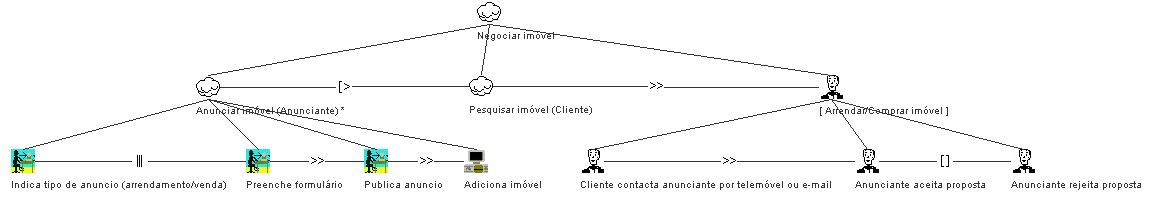
\includegraphics[width=1.2\textwidth]{images/Tarefas/geral_antes_Home4All_main}}

    \vspace{0.4cm}
    
    \makebox[\textwidth][c]{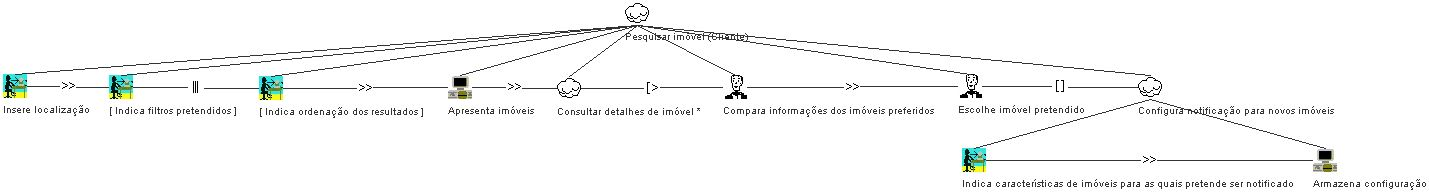
\includegraphics[width=1.2\textwidth]{images/Tarefas/geral_antes_Home4All_pesquisarImovel}}
    
    \vspace{0.1cm}
    
    \makebox[\textwidth][c]{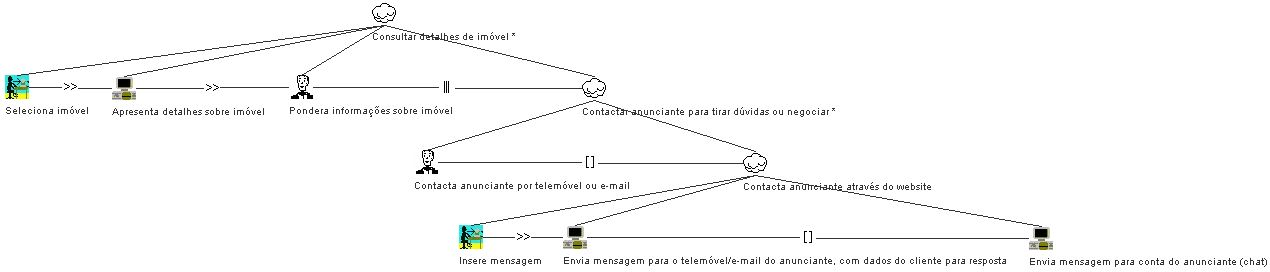
\includegraphics[width=1.2\textwidth]{images/Tarefas/geral_antes_Home4All_detalhesImovel}}

    \caption{Modelo de tarefas para negociar um imóvel, sem o \textit{website} \texttt{Home4All}.}
    \label{fig:modelo_tarefas_antes}
\end{figure}


\subsubsection{Com a aplicação \textit{web} \texttt{Home4All}}

De forma a compreender melhor as funcionalidades disponibilizadas para cada tipo de utilizador quando se utiliza o \texttt{Home4All}, desenvolveu-se o diagrama de \textit{use cases} apresentado na figura \ref{fig:use_cases}. Salienta-se que o ator \texttt{Utilizador} corresponde ao utilizador comum do \textit{website}, que pode ser um anunciante e um cliente simultaneamente.

\begin{figure}[H]
    \centering
    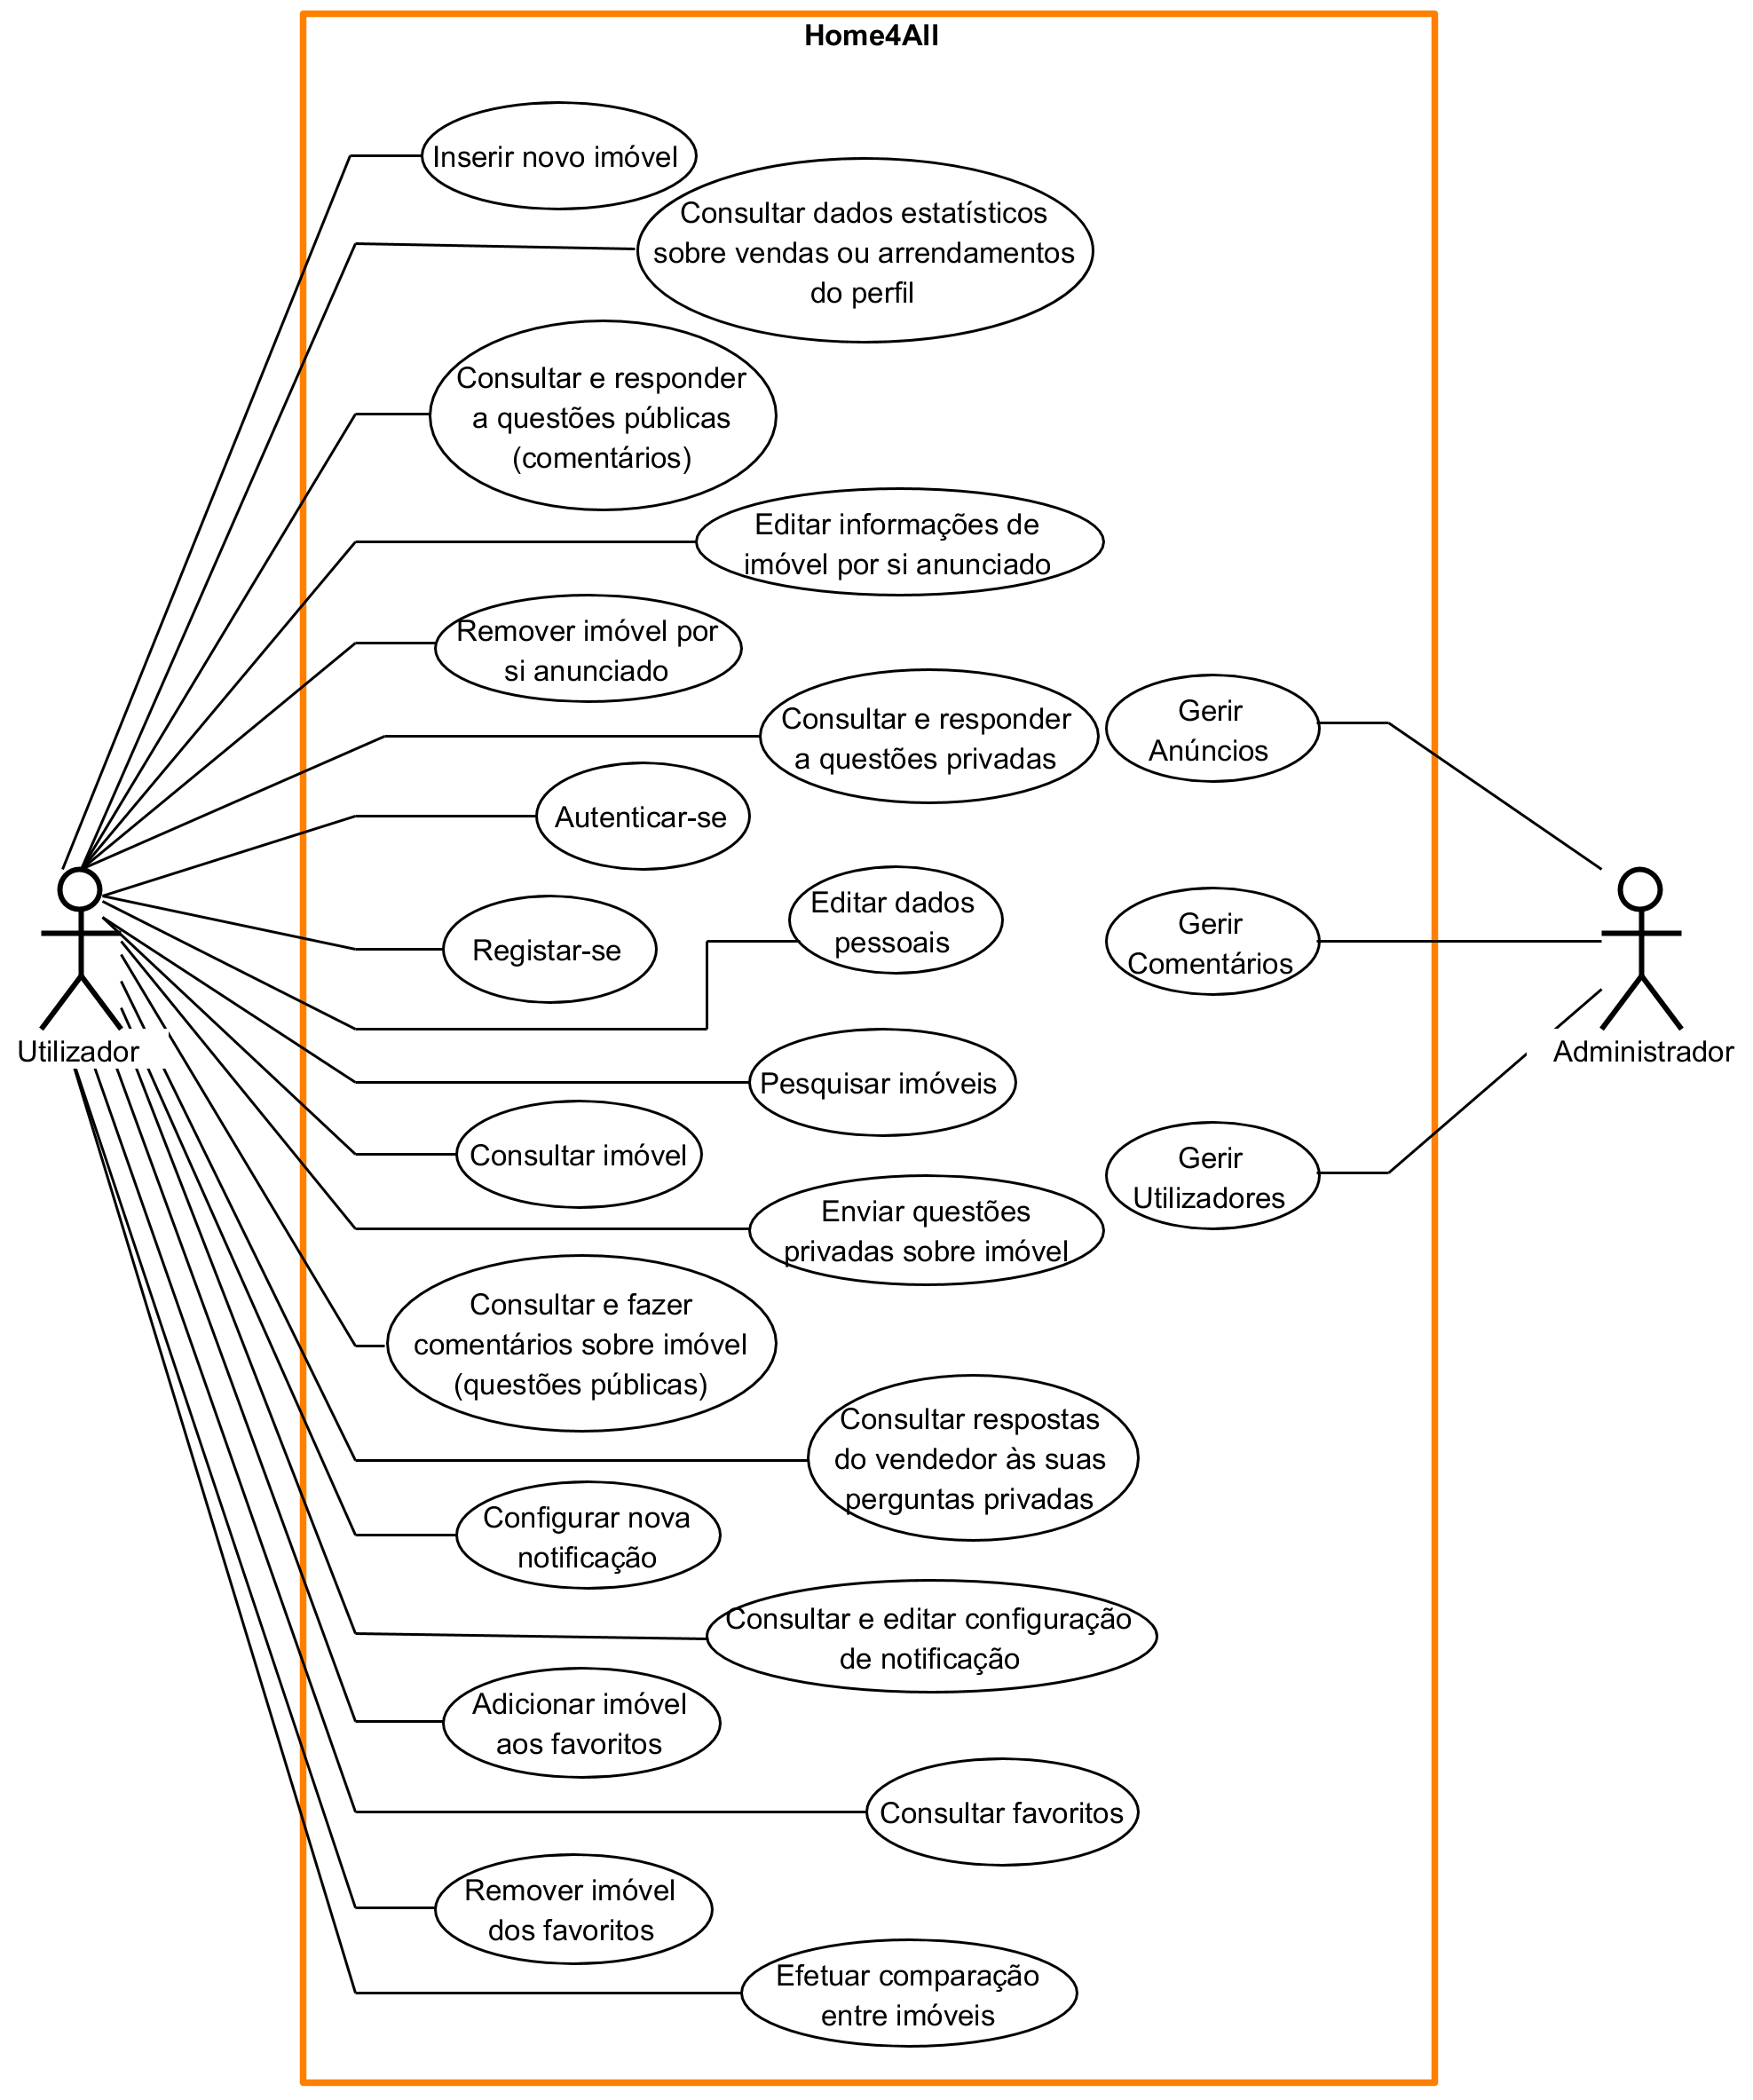
\includegraphics[width=0.9\textwidth]{./images/UseCases}
    \caption{Diagrama de \textit{use cases} do sistema \texttt{Home4All}}
    \label{fig:use_cases}
\end{figure}

Para além disso, construiu-se um modelo de tarefas geral, que descreve todo o processo de anúncio, pesquisa e compra/aluguer de imóvel, bem como o encadeamento de tarefas associadas. Este modelo é apresentado na figura \ref{fig:modelo_tarefas_depois}.

\begin{figure}[H]
    \centering
    \makebox[\textwidth][c]{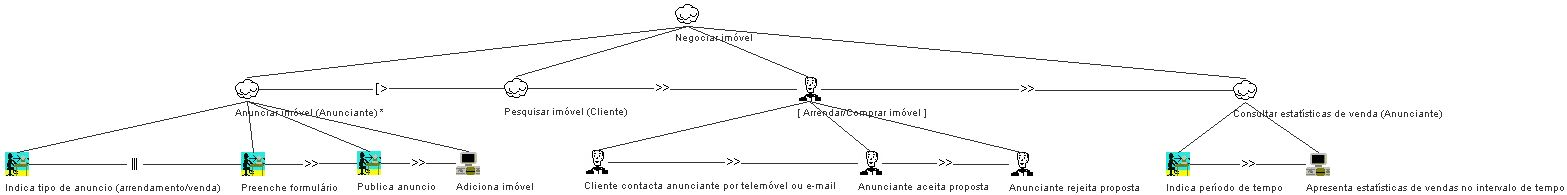
\includegraphics[width=1.2\textwidth]{images/Tarefas/geral_depois_Home4All_main}}

    \vspace{0.4cm}
    
    \makebox[\textwidth][c]{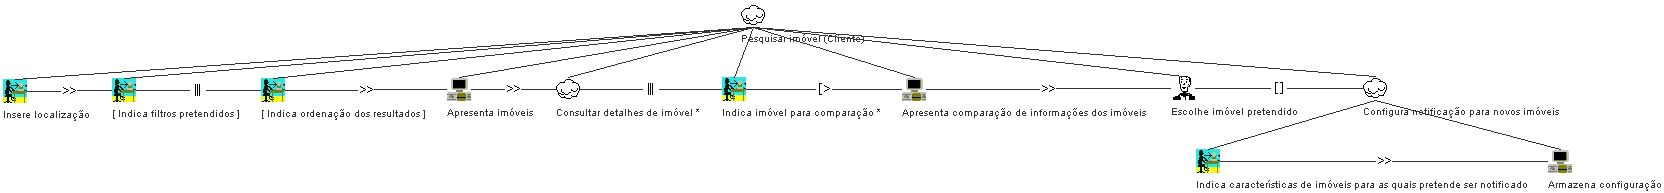
\includegraphics[width=1.2\textwidth]{images/Tarefas/geral_depois_Home4All_pesquisarImovel}}
    
    \vspace{0.1cm}
    
    \makebox[\textwidth][c]{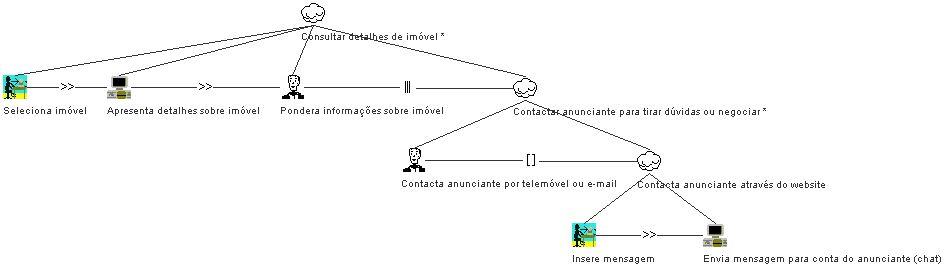
\includegraphics[width=1.2\textwidth]{images/Tarefas/geral_depois_Home4All_detalhesImovel}}

    \caption{Modelo de tarefas para negociar um imóvel, com o \textit{website} \texttt{Home4All}.}
    \label{fig:modelo_tarefas_depois}
\end{figure}

Destacam-se como principais melhorias neste modelo de tarefas geral, em relação ao modelo referente à utilização de outros \textit{websites}, o facto da comparação entre imóveis ser efetuada pelo sistema, facilitando o trabalho do utilizador. Para além disso, acrescenta-se a possibilidade de consulta de estatísticas de vendas, que pode ser útil para agentes imobiliários, por exemplo.

Salienta-se ainda que se espera implementar filtros bastante mais específicos em relação a outros \textit{websites}, o que permitirá tornar mais rápida e direta a pesquisa do cliente.

As principais tarefas desta aplicação são as de inserção de um novo imóvel, pesquisa de imóvel e comparação entre imóveis. Assim, apresenta-se os modelos dessas tarefas nas figuras \ref{fig:hat_vender}, \ref{fig:hat_arrendar} e \ref{fig:hat_comparar}.

\begin{figure}[H]
    \centering
    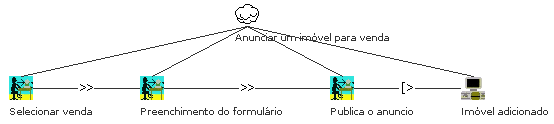
\includegraphics[width=0.8\textwidth]{images/Tarefas/hta_vender}
    \caption{Modelo da tarefa ``Anunciar imóvel para venda''}
    \label{fig:hat_vender}
\end{figure}

\begin{figure}[H]
    \centering
    \makebox[\textwidth][c]{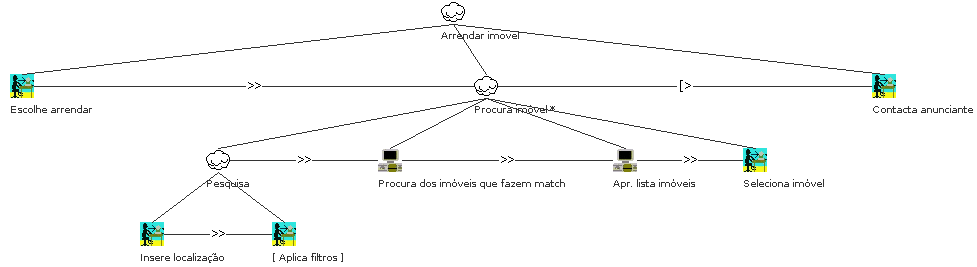
\includegraphics[width=1.2\textwidth]{images/Tarefas/hta_arrendar}}
    \caption{Modelo da tarefa ``Arrendar imóvel''}
    \label{fig:hat_arrendar}
\end{figure}

\begin{figure}[H]
    \centering
    \makebox[\textwidth][c]{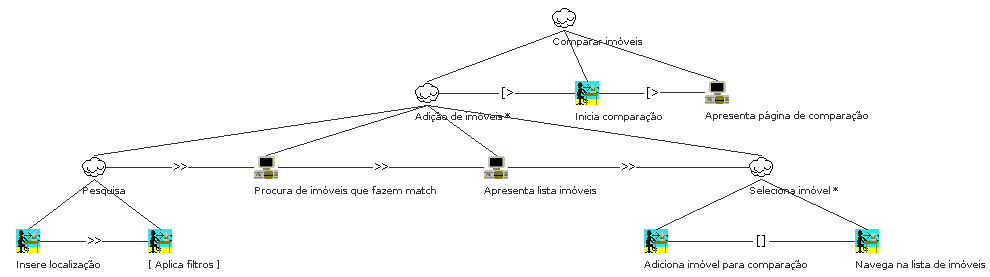
\includegraphics[width=1.2\textwidth]{images/Tarefas/hta_comparar}}
    \caption{Modelo da tarefa ``Comparar imóveis''}
    \label{fig:hat_comparar}
\end{figure}

